\documentclass{knowdive}
\usepackage{color,soul}
\usepackage{subcaption}
\usepackage{fancyhdr}
\usepackage{lastpage}
\usepackage{textcomp}
\usepackage{lscape}
\usepackage{rotating}
\usepackage{multirow}
\usepackage{listings}
\usepackage[table,xcdraw]{xcolor}
\usepackage{amsmath}
\usepackage{float}
\usepackage{graphicx}
\usepackage{enumerate}
\usepackage{hyperref}
\usepackage{rotating}
\usepackage{tabularx}
\graphicspath{ {images/} }

\usepackage{titlesec}
\titleformat{\section}{\LARGE\bfseries}{\thesection}{1em}{}

\newcommand{\mycomment}[1]{}

\lstset{%
    basicstyle=\normalsize\ttfamily,
    morecomment=[l][\color{gray}]{//},
}

\usepackage{array, makecell}
%\hypersetup{
	%pdfauthor={Author1, \and Author2},
	%pdftitle={Collectives.State of the Art},
       %pdfkeywords = {},
      %pdfsubject={}
      %}
%\usepackage{hyperref}

\newcolumntype{M}[1]{>{\arraybackslash}m{#1}}
\graphicspath{ {images/} }
\usepackage{comment}

\title{KGE 2024 Project\\\vspace{0.2cm}Sport Facilities \& Events in Trentino}

\author{Christian Sassi, Pietro Bologna, Mouez Khelifi}

\revisionhistory{
    \revision{0.1}{October 16, 2024}{Christian Sassi, Pietro Bologna}{Document created}
    \revision{1.1}{October 25, 2024}{Christian Sassi, Pietro Bologna}{Purpose definition phase}
    \revision{1.2}{October 29, 2024}{Christian Sassi, Pietro Bologna}{Revision of purpose definition phase}
    \revision{1.3}{November 6, 2024}{Christian Sassi, Pietro Bologna, Mouez Khelifi}{Correction to ER model and PF Sheet}
    \revision{2.1}{November 7, 2024}{Christian Sassi, Pietro Bologna, Mouez Khelifi}{Information Gathering phase}
    \revision{2.2}{November 9, 2024}{Christian Sassi, Pietro Bologna, Mouez Khelifi}{Dataset collection}
    \revision{2.3}{November 13, 2024}{Christian Sassi, Pietro Bologna, Mouez Khelifi}{Revision of information gathering phase}  
    \revision{3.1}{November 20, 2024}{Christian Sassi, Pietro Bologna, Mouez Khelifi}{Language Definition phase}
    \revision{3.2}{November 21, 2024}{Christian Sassi, Pietro Bologna, Mouez Khelifi}{Revision of language definition phase}  
    \revision{4.1}{November 21, 2024}{Christian Sassi, Pietro Bologna, Mouez Khelifi}{Knowledge Definition phase}
}
\newpage

\fancypagestyle{plain}{
  \fancyhf{}% Clear header/footer
  %\fancyhead[R]{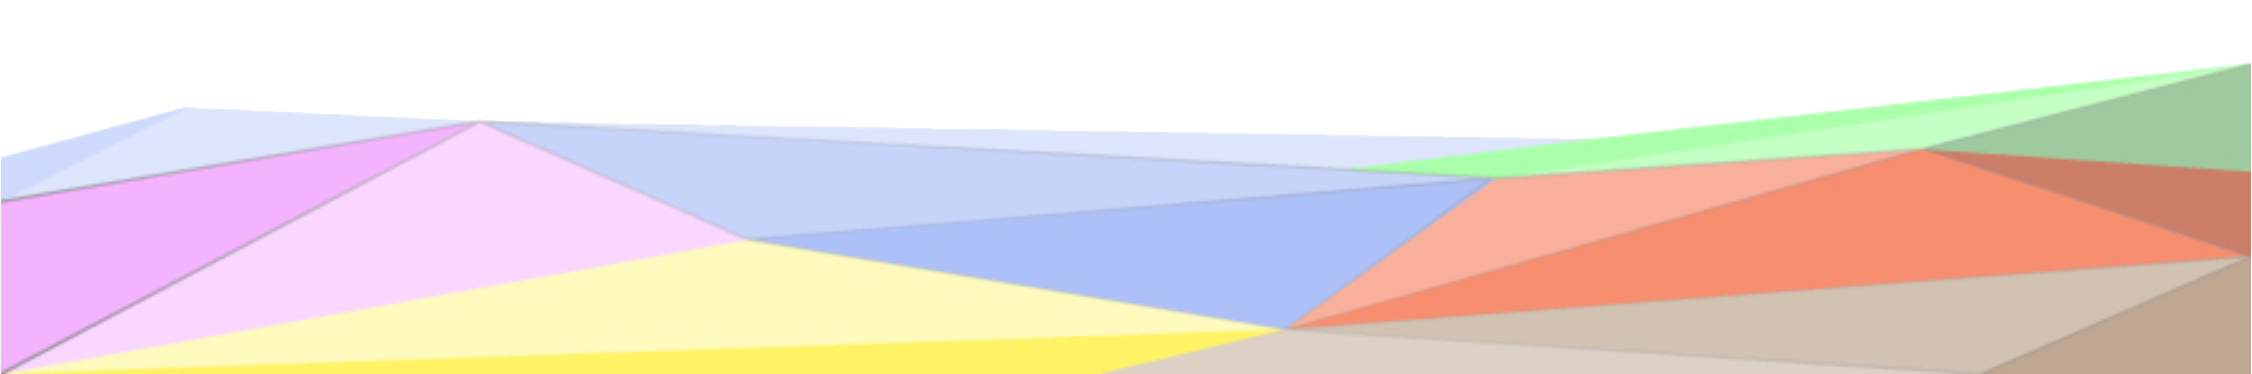
\includegraphics[width=1.0\linewidth,height=5pt]{Knowdive_color_bar}}% Right header
  \fancyfoot[L]{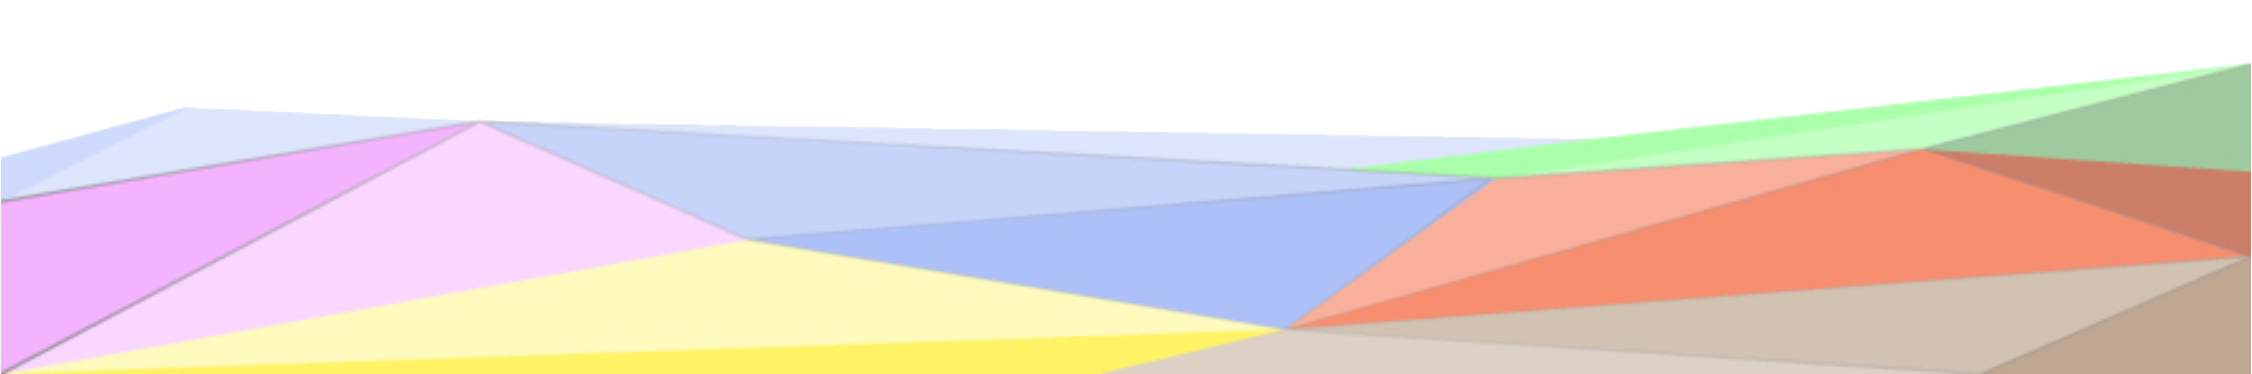
\includegraphics[width=1.0\linewidth,height=45pt]{Knowdive_color_bar}}% Left footer
  \fancyfoot[C]{Page \thepage\  / \pageref{LastPage}}
}

\pagestyle{plain}
%\makeglossaries
%input{glossaries}
\begin{document}

\maketitle
\begin{sloppypar}

\large
\begin{spacing}{1.05}
%\gls{latex}
%\gls{batex}
%\gls{eType}
%\printglossary

\section{Introduction}

\noindent Access to sports facilities and related events is essential for enhancing the quality of life in modern cities and regions. In areas like Trentino Province, providing convenient access to a range of sports infrastructure and events is increasingly important for both residents and visitors. Promoting an active lifestyle and supporting community-driven initiatives are key to strengthening the livability of the region.\\

\noindent To address these needs, we present a project for the Knowledge Graph Engineering course, integrating data on sports facilities and events in Trentino. This Knowledge Graph will offer citizens, tourists, and local authorities a comprehensive, interconnected view of available sports facilities, and related sport events. By combining data on facilities and events, the Knowledge Graph will empower users to make informed decisions that enhance community participation, public health, and the region’s sporting culture.\\

\noindent Reusability is one of the main principles in the Knowledge Graph Engineering (KGE) process defined by iTelos. The KGE project documentation plays an important role to enhance the reusability of the resources handled and produced during the process. A clear description
of the resources as well as of the process (and single activities) developed, provides a clear understanding of the project, thus serving such an information to external readers for the future exploitation of the project’s outcomes.\\

\noindent The current document aims to provide a detailed report of the project developed following the iTelos methodology. The report is structured as follows:
\begin{itemize}
    \item Section 2: Definition of the project's purpose and its domain of interest.

    \item Section 3: High level description of the project development, based on the Produce role's objectives.  
    
    \item Sections 4, 5, 6, 7 and 8: The description of the iTelos process phases and their activities, divided by knowledge and data layer activities.
    
    \item Section 9: The description of the evaluation criteria and metrics applied to the project final outcome.

    \item Section 10: The description of the metadata produced for all (and all kind of) the resources handled and generated by the iTelos process, while executing the project.

    \item Section 11: Conclusions and open issues summary.
\end{itemize}

\noindent You can access the GitHub repository, which contains all the materials used during the project's development, via this \href{https://github.com/christiansassi/knowledge-graph-engineering-project}{link}.
\section{Purpose Definition}
\noindent Access to sports facilities and events has a significant impact on the quality of life in regions like Trentino Province. Reliable information on the availability and accessibility of these resources can inspire a more active lifestyle and enhance community engagement. The \textbf{purpose} of this project is to develop a Knowledge Graph that consolidates information on sports facilities and events in Trentino, creating a unified resource for residents, tourists, and local authorities. By providing a comprehensive overview, the Knowledge Graph supports informed decision-making, promotes community involvement, enhances public health, and cultivates a vibrant sports culture in the region.

\subsection{Informal Purpose}
% The informal Purpose: a natural language sentence expressed by the iTelos user (usually the Domain Expert), which state the objective for which the iTelos methodology needs to be applied. Example: ”I want to build a KG that represents how the environmental impact in Italy has changed over the last five years and what actions in my life have an impact on this.”
We want to build a Knowledge Graph that brings together all the information on sports facilities and events across Trentino. The goal is to make it easy for people to find sports venues, check out upcoming events, and get involved in physical activities. By offering details on what facilities are available, when events are happening, and what kinds of sports are offered, this project aims to promote an active lifestyle. Ultimately, we want this Knowledge Graph to be a go-to resource for anyone looking to make informed decisions about sports and activities in the region.

% Domain of interest: It refers to the area of knowledge or field of study of interest.
\subsection{Domain of Interest (DoI)} 
After analyzing the purpose, the next step is to define the Domain of Interest (DoI). The DoI provides details about the geographical area and time frame relevant to the project purpose. The Domain of Interest for this project is as follows: 
\begin{itemize} 
    \item The \textbf{geographical space} for this project is defined by the administrative boundaries of the Trentino Province. We ensure that only sports facilities and centers located within this region are included in our dataset, encompassing both urban and rural locations where sports facilities, such as soccer fields, tennis courts, basketball courts, and other venues, are situated. Additionally, this geographical space applies to the sports events data, ensuring that all events included are those taking place within the Trentino Province. Many of these events are based on those organized for the Festival dello Sport 2024, which brings a concentrated focus on sports culture and activities within one of the main city of the region. 
    \item The \textbf{temporal domain} for this project is focused on the year 2024. The data on sports facilities and events reflects the information available for this specific period, capturing the current landscape of sports resources and scheduled events within Trentino Province throughout the year. 
\end{itemize}

\subsection{Scenarios definition}
Here we define a set of usage scenarios, describing the multiple aspects considered by the project purpose. Four key scenarios are considered:
\begin{enumerate}
    \item \textbf{Weekday}: Across the Trentino, on a typical weekday.
    \item \textbf{Weekend}: In the province of Trento, on a weekend, when sports facilities may see an higher activity as locals and tourists alike participate in and spectate at community sports events. 
    \item \textbf{Holidays}: In Trentino, during the holiday periods (e.g. Christmas, Summer, etc.), when a high influx of tourists is expected.
    \item \textbf{Festival dello Sport:} In Trento, during the \textit{Festival dello Sport 2024}. During this time, a variety of sports events and exhibitions are scheduled, attracting both residents and visitors. 
\end{enumerate}

\subsection{Personas}
Now, we define a set of real users acting within the scenarios defined above. Each Persona is defined over a specific features included in the main purpose.
\begin{enumerate}
    \item \textbf{Luca} is a 35-year-old engineer working in Trento. He is passionate about outdoor sports, especially padel.
    % After work, he enjoys playing outdoor sports like tennis and often looks for additional activities to participate in. , but frequently struggles to find suitable events. 
    \item \textbf{Anna} is a 21-year-old university student from Verona, studying in Trento. She enjoys playing volleyball with her friends.
    % Additionally, she is interested in attending related events. % but finds it challenging to discover suitable options.
    \item \textbf{Matteo} is a 42-year-old tourist visiting Trento during the Christmas holidays. He has a passion for winter sports.
    % He seeks out local events and activities, such as skiing and snowboarding, to make the most of his visit.
    \item \textbf{Camilla} is a 24-years-old a volunteer student at the annual "Festival dello Sport" in Trento and assist visitors discovering the wide range of activities available throughout the city. 
    % During the festival, she relies on this service to keep track of the event schedule, locate different demonstrations and workshops, and 
\end{enumerate}

\subsection{Competency Questions (CQs)}
From the above information, here we have the list of Competency Questions (CQs) created considering the personas in the defined scenarios.
\begin{enumerate} 
    \item \textbf{CQ1}: Luca inquires about available padel courts in Trento after 7 PM.
    \item \textbf{CQ2}: Luca also asks if there are any padel events during the weekend of the Festival dello Sport.
    \item \textbf{CQ3}: Luca asks if there will be events in Trentino that have Sara Errani as a guest.
    \item \textbf{CQ4}: Anna wants to know what sports can be practiced in Trentino.
    \item \textbf{CQ5}: Spending the weekend with friends in Folgaria, Anna asks if there are any lighted volleyball or beach volleyball courts available throughout the day.
    \item \textbf{CQ6}: As a volleyball enthusiast, Anna would like to know if there will be any volleyball events during the summer holidays of 2024.
    \item \textbf{CQ7}: Matteo also wants to know if there are any skiing events held in Stelvio National Park during the winter season.
    \item \textbf{CQ8}: Not finding what he’s looking for, Matteo asks if there are any sport events during his vacation in Trentino.
    \item \textbf{CQ9}: A visitor asks Camilla about the events happening today, October 10, at the Festival dello Sport.
    \item \textbf{CQ10}: While volunteering at the Festival dello Sport, Camilla becomes interested in tennis and wants to know if there are any tennis-related events and if tennis courts are available when she returns to Molveno for the weekend. 
\end{enumerate}

\subsection{Concepts identification}
From the scenarios, personas and CQs we extract the following entities with their properties:
\begin{figure}[H]
    \centering
    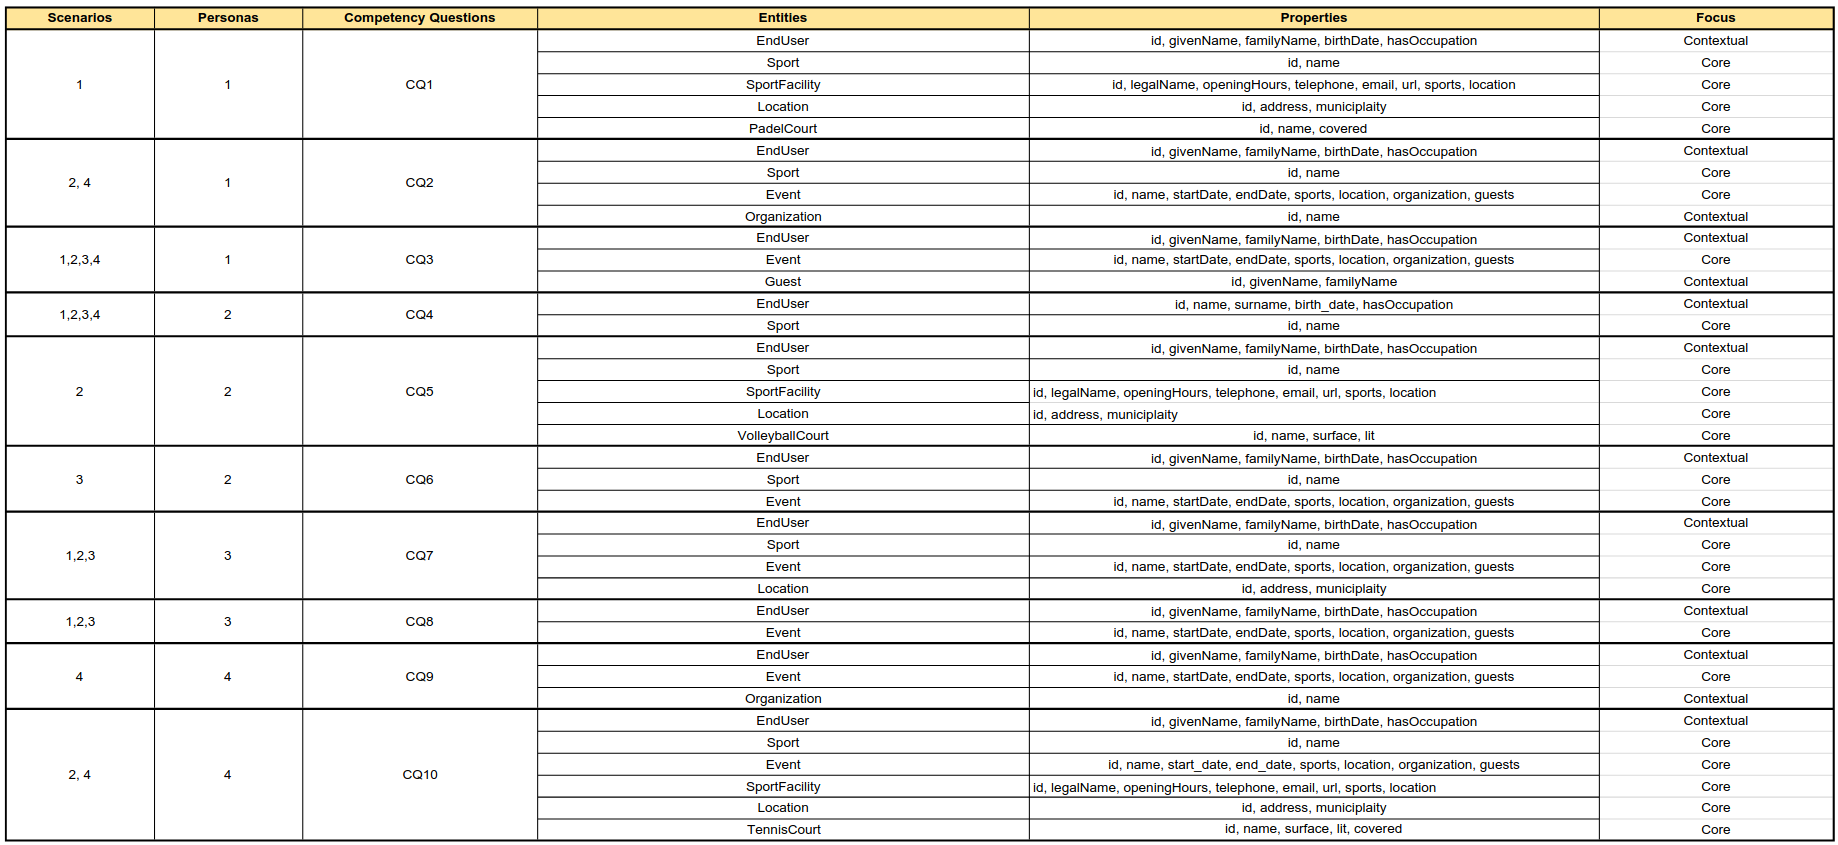
\includegraphics[width=1\linewidth]{knowdive-files/PFSheet.png}
    \caption{PF Sheet}
    \label{fig:concepts_identification}
\end{figure}

\subsection{ER model definition}
The ER diagram, which graphically represents the knowledge gathered in the prior stages. This ER diagram provides detailed information for a technician to delve deeper into the project. The diagram is based on the entity types (ETypes) and attributes identified before.
\begin{figure}[H]
    \centering
    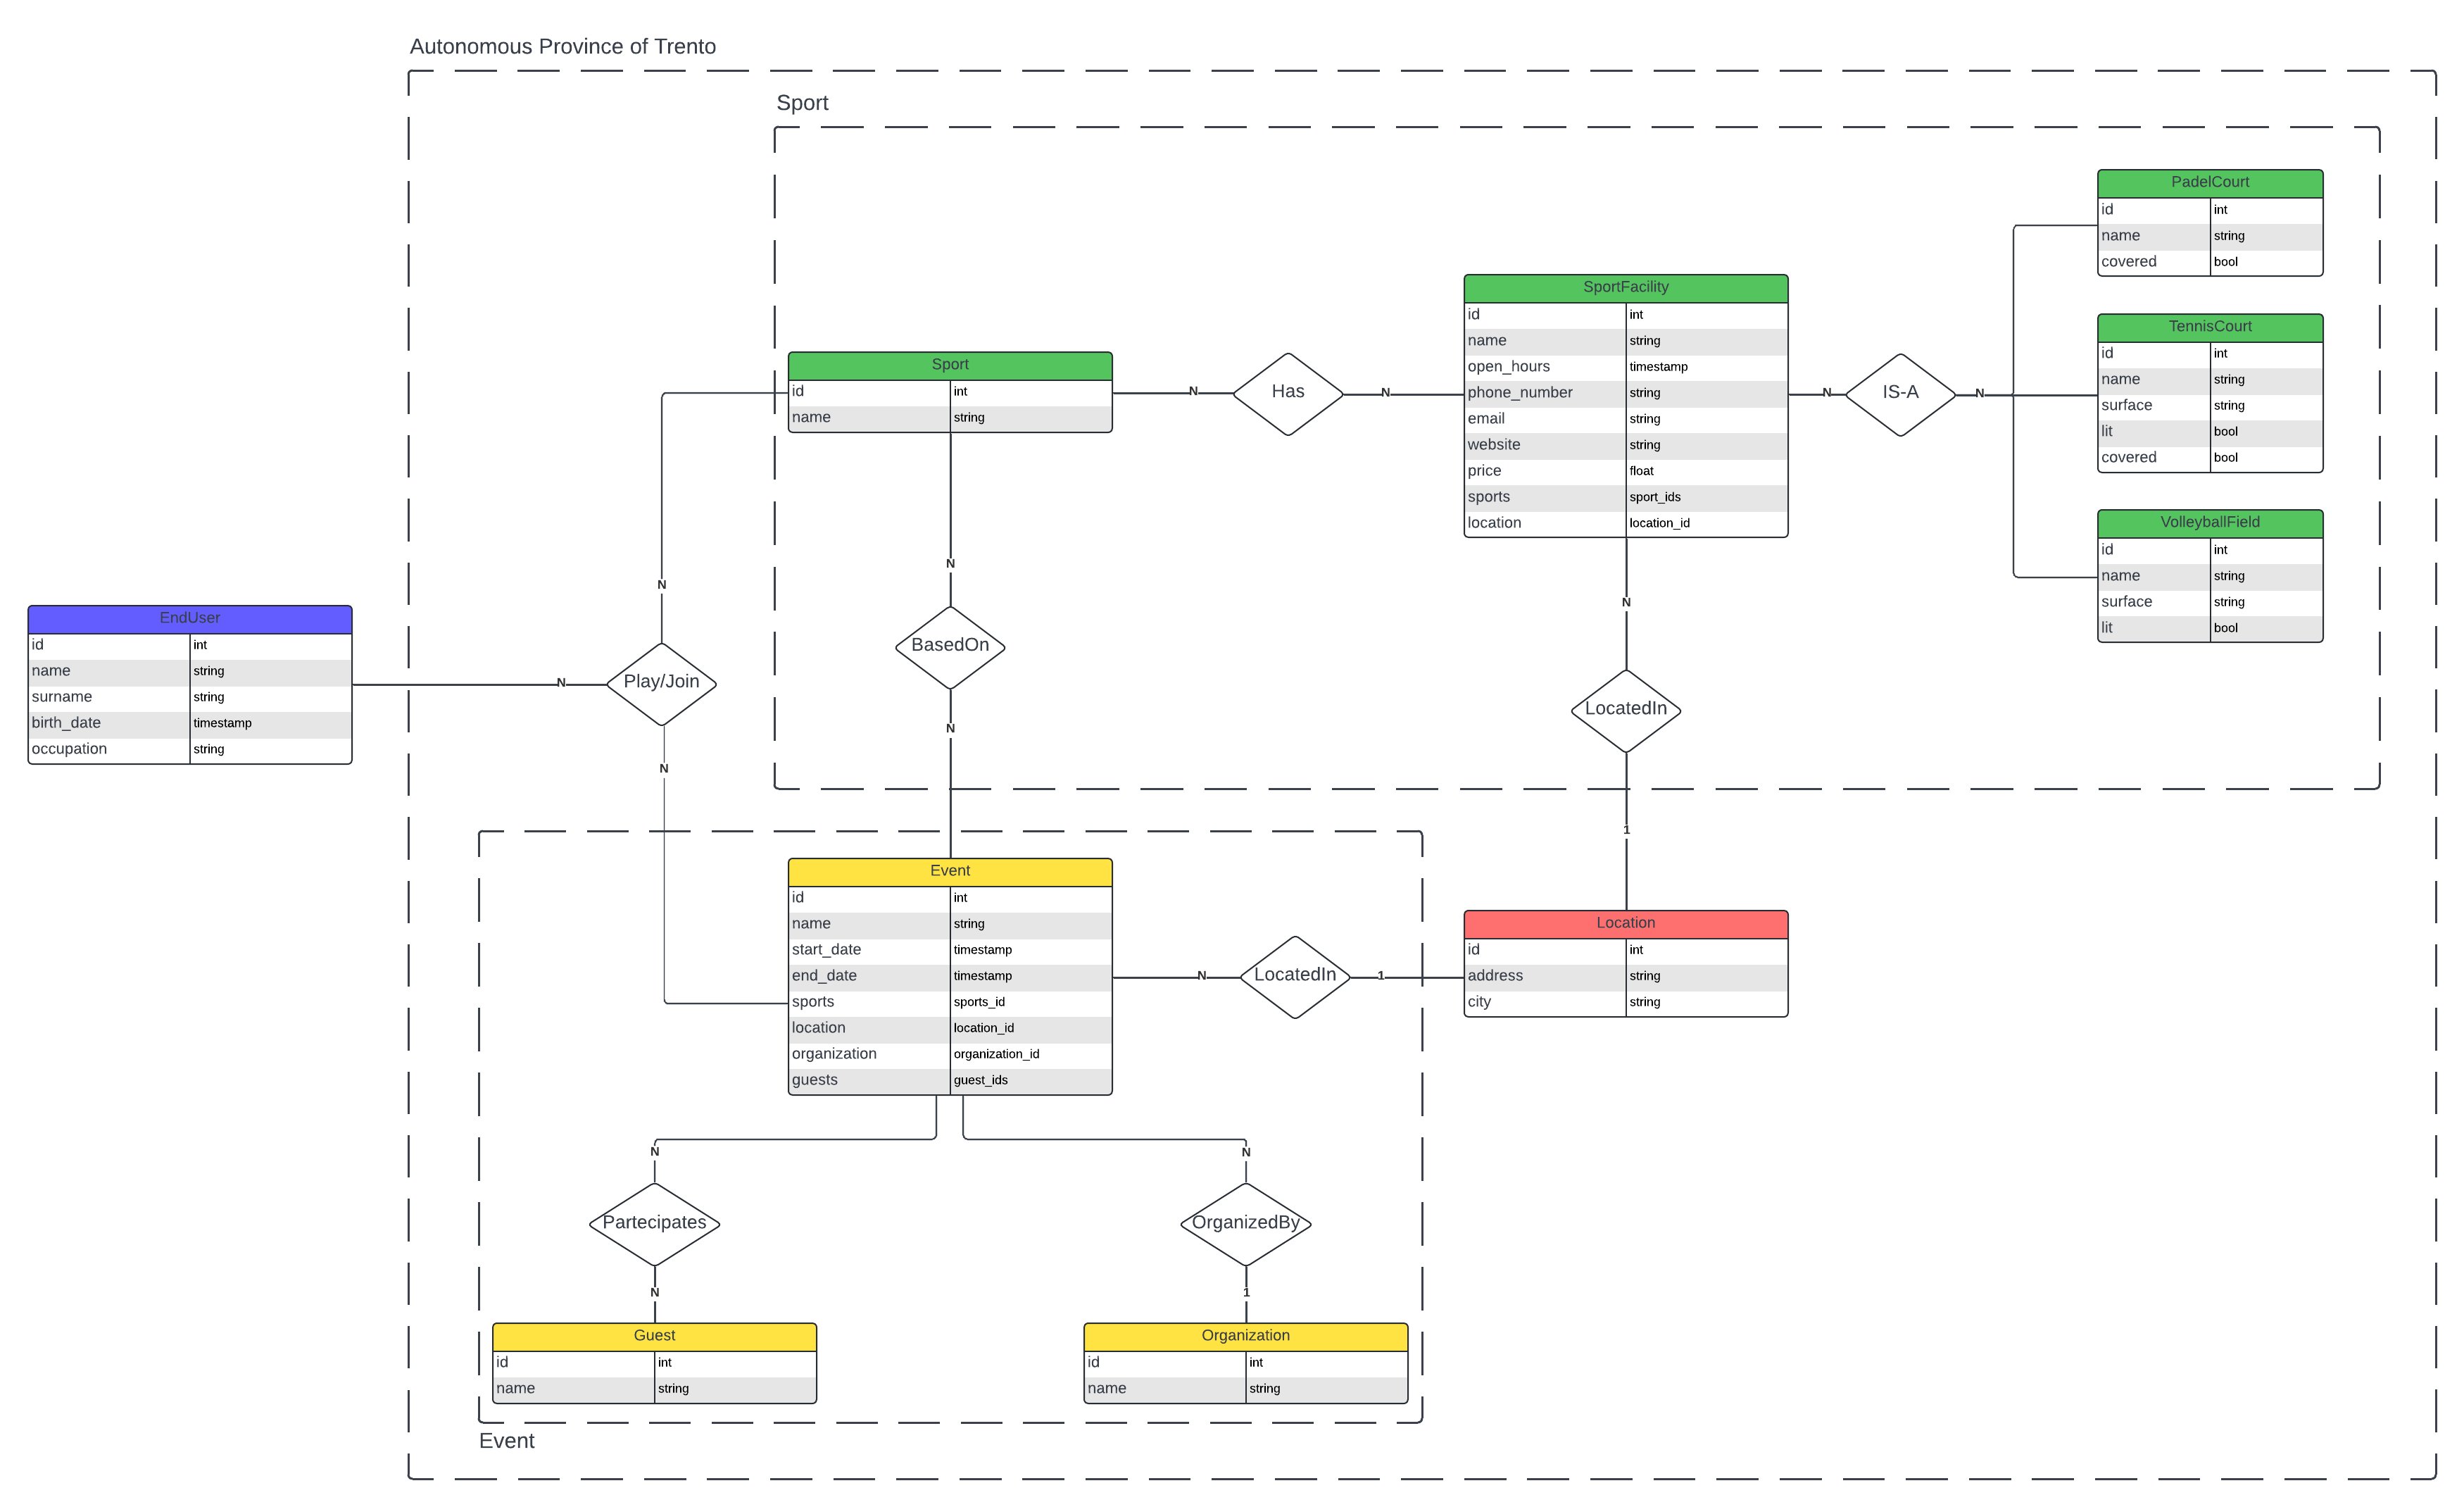
\includegraphics[width=1\linewidth]{knowdive-files/ER_model.png}
    \caption{ER model}
    \label{fig:er_model}
\end{figure}

\noindent The following ETypes shown in Figure \ref{fig:er_model} have been identified to illustrate how the different entities interact within the model, providing a clear and coherent structure for representing information about sports facilities and events in Trentino.\begin{enumerate}
    \item \textbf{SportFacility}: Represents a facility dedicated to sports, where individuals can participate in various physical activities.
    \begin{itemize}
        \item \texttt{id}: Unique identifier for each sports facility.
        \item \texttt{legalName}: Name of the sports facility.
        \item \texttt{openingHours}: Operating hours for the facility.
        \item \texttt{telephone}: Contact phone number for the facility.
        \item \texttt{email}: Contact email address for the facility.
        \item \texttt{url}: Website link for more information.
        \item \texttt{sports}: List of sports available at the facility, linked to sport IDs.
        \item \texttt{location}: Address or general location information.      
    \end{itemize}

    \item \textbf{PadelCourt}: A court dedicated to padel, a racquet sport.
    \begin{itemize}
        \item \texttt{id}: Unique identifier for the padel court.
        \item \texttt{name}: Name of the padel court.
        \item \texttt{covered}: Indicates if the court is covered.
    \end{itemize}

    \item \textbf{TennisCourt}: A court dedicated to tennis.
    \begin{itemize}
        \item \texttt{id}: Unique identifier for the tennis court.
        \item \texttt{name}: Name of the tennis court.
        \item \texttt{surface}: Type of surface on the court (e.g., clay, grass).
        \item \texttt{lit}: Indicates if the court has lighting.
        \item \texttt{covered}: Indicates if the court is covered.
    \end{itemize}

    \item \textbf{VolleyballField}: A field dedicated to volleyball.
    \begin{itemize}
        \item \texttt{id}: Unique identifier for the volleyball field.
        \item \texttt{name}: Name of the volleyball field.
        \item \texttt{surface}: Type of surface on the field (e.g., sand, grass).
        \item \texttt{lit}: Indicates if the field has lighting.
    \end{itemize}

    \item \textbf{Sport}: Represents a specific type of sport.
    \begin{itemize}
        \item \texttt{id}: Unique identifier for each sport.
        \item \texttt{name}: Name of the sport.
    \end{itemize}

    \item \textbf{Event}: Represents an organized sports event, including details on participation and scheduling.
    \begin{itemize}
        \item \texttt{id}: Unique identifier for each event.
        \item \texttt{name}: Name of the event.
        \item \texttt{startDate}: Start date of the event.
        \item \texttt{endDate}: End date of the event.
        \item \texttt{sports}: Sports included in the event, linked to sport IDs.
        \item \texttt{location}: Location where the event is held, linked to location ID.
        \item \texttt{organization}: Organization responsible for the event, linked to organization ID.
        \item \texttt{guests}: List of guest participants, linked to guest IDs.
    \end{itemize}

    \item \textbf{Guest}: Represents a guest or participant involved in a sports event.
    \begin{itemize}
        \item \texttt{id}: Unique identifier for each guest.
        \item \texttt{givenName}: The first name of the guest.
        \item \texttt{familyName}: The last name of the guest.
    \end{itemize}

    \item \textbf{Organization}: Represents an organization responsible for hosting or coordinating sports events.
    \begin{itemize}
        \item \texttt{id}: Unique identifier for each organization.
        \item \texttt{name}: Name of the organization.
    \end{itemize}

    \item \textbf{Location}: Represents a physical location where sports facilities and events are held.
    \begin{itemize}
        \item \texttt{id}: Unique identifier for each location.
        \item \texttt{address}: Full address of the location.
        \item \texttt{municipality}: City in which the location is situated.
    \end{itemize}

    \item \textbf{EndUser}: Refers to the end user who will utilize the service..
    \begin{itemize}
        \item \texttt{id}: Unique identifier for each user.
        \item \texttt{givenName}: The first name of the end user.
        \item \texttt{familyName}: The last name of the end user.
        \item \texttt{birthDate}: Birth date of the user.
        \item \texttt{hasOccupation}: The person's occupation.
    \end{itemize}
\end{enumerate}

\noindent This ER model is also structured around several relationships:
\begin{enumerate}
    \item \textbf{Placed}: It contextualizes where the facilities and events are physically situated, allowing users to identify precise addresses or areas for sports facilities and event venues.
    \item \textbf{Has}: It defines the kinds of sports activities or facilities available within each SportFacility, supporting users in finding facilities based on specific sports or equipment.
    \item \textbf{IS-A}: It allows the model to recognize these entities as specific kinds of SportFacility, enabling queries about both general facilities and specific facility types, based on shared attributes.
    \item \textbf{Organise}: It identifies the entity responsible for organizing an event, allowing users to find events hosted by specific organizations or understand the event’s affiliation.
    \item \textbf{Appear}: It enables user queries about the guest lists.
    \item \textbf{BasedOn}: Identifies the sport associated with an event.
    \item \textbf{Play}: Indicates the sport played by the user.
    \item \textbf{Attend}: Indicates the event joined by the user.
\end{enumerate}

\noindent Due to the broad accessibility of the sports world, we decided not to focus solely on the university domain; instead, we envisioned this service as accessible to everyone in Trentino. \ Building on this idea, our goal became developing a service capable of helping citizens find relevant sports events and facilities throughout Trentino.

\noindent From a temporal perspective, we chose to support requests specific to the year 2024, while from a geographical perspective, we based our service on the entire Trentino region. \\
Both these temporal and geographical choices have their strengths and weaknesses. Regarding the temporal choice, the main limitation is that we are restricted to the year 2024, as sports events data from previous years is often incomplete or inconsistent, with some years missing data entirely. Looking forward, another limitation is that our service remains fixed to 2024, as we cannot guarantee that future data providers will address these critical gaps in coverage. By focusing on 2024, however, we ensure that our service operates reliably, leveraging a dataset we know to be comprehensive—this is a major strength of our approach. \\
As for the geographical choice, as outlined in our purpose definition, our service is designed to function across the entire Trentino region, making it one of the service’s greatest strengths. However, it is important to note that for some entities, especially sports facilities, certain fields may be missing, such as contact information—particularly for less documented facilities. This also applies to specific types of facilities, such as volleyball fields, where some sports facilities may have incomplete data. Despite these gaps, we chose to model these properties because they align with the project’s purpose: providing a complete and unified view of sports facilities and events in the region. By including these attributes in the model, we establish a structure that can accommodate future data as it becomes accessible. This approach ensures that the Knowledge Graph can be expanded and refined over time, allowing it to better serve the needs of residents, tourists, and local authorities seeking information about sports opportunities in Trentino.

% ----------------------------------------------------------------------------------- %
\mycomment{
The Purpose Definition section has to report the process activities included in the first phase of the iTelos methodology, as well as the results achieved. More in details a description of the below components is required:
\begin{itemize}
    \item \textbf{Informal Purpose}: as main input for the project the initial statement describing informally the project purpose has to be reported.
    \item  \textbf{Domain of Interest (DoI)}: the domain in which the purpose is considered. The DoI has to be described in terms of space and time constraints, plus a description of its main features. The DoI description informs the reader about the geographical space, as well as the period of time, in which the project purpose is considered.
    \item \textbf{Scenarios definition}: a set of usage scenarios, describing the multiple aspects considered by the project purpose.
    \item \textbf{Personas}: a set of real users acting  within the scenarios defined above. Each Persona is defined over a specific features included in the main Purpose.  
    \item \textbf{Competency Questions (CQs)}: the list of CQs created considering the personas in the scenarios defined.
\end{itemize}

\noindent The above steps aim at catching the diversity expressed by the project purpose, by defining clearly the different aspects, about the involved contexts and actors. To this end, while describing the above activities the writer has to report those scenarios, personas and questions, whose better describe all the several and diverse aspects of the project purpose.\\

\noindent For the remaining two activities of the first iTelos phase, the writer has to specify which formal elements (entities and properties) can be extracted from the above definitions, and how they interact together with the objective of satisfying the project purpose. 
        
\begin{itemize}
    \item \textbf{Concepts identification}: the terms representing the entities, and their properties, to be consider in the KGE project, classified using the popularity categories.
    \item  \textbf{ER model definition}: the entities and property identified in the step above, are used to design the purpose ER model. this is the last step of the purpose formalization process.
\end{itemize}

\noindent The report of the work done during the first phase of the methodology, has to includes also the description of the  different choices made, with their strong and weak points. In other words the report should provide to the reader, a clear description of the reasoning conducted by all the different team members.\\
}



\section{Information Gathering}
Information gathering is the second phase in the iTelos methodology for knowledge graph engineering. This phase involves collecting and processing the resources needed to build the final Entity Graph (EG), following the purpose defined in the first phase. The process works with three types of datasets: data value datasets, knowledge datasets (ontologies), and language datasets. Beyond just collecting data, this phase aims to improve the quality and reusability of the gathered information through cleaning and standardization steps. This organized approach ensures the knowledge graph is built using high-quality, compatible data that effectively meets its intended purpose.

\subsection{Sources identification}
The first activity within the Information Gathering phase involves identifying and accessing relevant sources of information. This step includes examining the input sources provided and potentially exploring additional sources if the initial inputs prove insufficient.

\vspace{0.4cm}
\noindent The goal is to enable data reuse by locating pre-existing data sources that can provide the required information, by actively searching for datasets aligned with the project's objectives, ensuring the efficient use of available resources

\noindent Given the heterogeneous nature of data, multiple types of sources must be considered to effectively cover the diverse aspects of the project. To ensure high-quality and reliable information, the emphasis is placed on using "high-quality" sources, such as Pagine Gialle and catalogs of interoperable, reusable datasets. These sources are often maintained in repositories or live data catalogs (e.g., OpenData Trentino), where data and other relevant resources are published and made accessible.
\vspace{0.4cm}

\noindent\textbf{a. Data Layer\\}
\noindent The Data Layer encompasses the diverse data sources used to populate and structure information about sports facilities and events in the Trentino region. The goal is to gather comprehensive, high-quality datasets that provide detailed and relevant information. The selected sources include publicly accessible datasets and online directories, ensuring broad coverage of the various aspects related to sports and recreation. 
\vspace{0.4cm}

\noindent Below is an overview of the primary data value sources utilized in this project:
\begin{enumerate}
    \item \textbf{Overpass Turbo}
    \begin{itemize}
        \item \textit{Description}: A web-based tool for querying OpenStreetMap (OSM) data, allowing detailed searches for features like sports facilities, parks, and roads using the Overpass API. Ideal for extracting geospatial data.
        \item \textit{Access Link}: \href{https://overpass-turbo.eu/}{overpass-turbo.eu}
    \end{itemize}

    \item \textbf{OpenData Trentino}
    \begin{itemize}
        \item \textit{Description}: The official Open Data Portal of Trentino, offering access to datasets across various sectors like transportation, tourism, and public services. Supports data reuse and innovation.
        \item \textit{Access Link}: \href{https://dati.trentino.it/dataset}{dati.trentino.it}
    \end{itemize}
    
    \item \textbf{Pagine Gialle}
    \begin{itemize}
        \item \textit{Description}: An online directory of businesses in Italy, categorized by industry. Provides contact details, addresses, and user reviews for services like restaurants and sports facilities.
        \item \textit{Access Link}: \href{https://www.paginegialle.it/}{paginegialle.it}
    \end{itemize}

    \item \textbf{Festival dello Sport}
    \begin{itemize}
        \item \textit{Description}: An annual sports event in Trento featuring panels, workshops, and live sports. It gathers athletes and sports enthusiasts, providing insights into the sports industry.
        \item \textit{Access Link}: \href{https://www.ilfestivaldellosport.it/programma/}{ilfestivaldellosport.it}
    \end{itemize}

    \item \textbf{Comune di Trento}
    \begin{itemize}
        \item \textit{Description}: The official website of Trento's municipal administration, offering information on public services, events, and datasets related to urban planning and local services.
        \item \textit{Access Link}: \href{https://www.comune.trento.it/Aree-tematiche/}{www.comune.trento.it}
    \end{itemize}

    \item \textbf{List of Municipalities}
    \begin{itemize}
        \item \textit{Description}: List of municipalities of Trentino province.
        \item \textit{Access Link}: \href{https://github.com/alihamzaunitn/kdi-educationtrentino/blob/master/Datasets/Data%20Integration/Trentino%20Commune%20List.csv}{github.com/alihamzaunitn/kdi-educationtrentino}
    \end{itemize}
    
\end{enumerate}
\noindent For this project, it wasn’t possible to determine if one data source was better than another. This is because, for the type of data we handle—especially event-related data—available resources were limited. Choosing between them would have left us with very little data or, in the worst case, none at all.
\vspace{0.4cm}

\noindent\textbf{b. Knowledge Layer\\}
\noindent In designing the Knowledge Layer for Sports Facilities and Events in Trentino, we initially considered using the \textbf{General Transit Feed Specification (GTFS)}, a standard for public transit data. However, as the project's focus is not on public transit schedules or routes, the GTFS schema was deemed unsuitable. Instead, we opted to use \href{https://schema.org/docs/schemas.html}{\textbf{Schema.org}}, which better aligns with the project's requirements and is more readily available for use. 

\vspace{0.4cm}
\noindent Additionally, some property names in our model do not strictly follow the Schema.org vocabulary. This deviation was necessary to better address the specific needs and purposes of our project. This custom adaptation ensures the Knowledge Graph accurately represents the context and requirements of project's purpose.

\subsection{Datasets collection}
The Data Collection phase focuses on acquiring relevant datasets to populate the project's knowledge base. This phase involves several key steps, including the selection of data sources, gathering the data, and ensuring its quality and completeness.
\vspace{0.4cm}

\noindent The data collection process employed three main approaches:
\begin{itemize}
    \item \textbf{Direct Downloads}: Some datasets, such as those available from \textit{OpenData Trentino}, were collected directly in formats like CSV or JSON. These datasets are freely downloadable, ensuring that they are immediately usable without requiring additional extraction steps. However, it should be noted that in some circumstances, especially for \textit{OpenData Trentino}, web scraping was necessary to gather these resources more efficiently and quickly.
    \item \textbf{API}: For sources like \textit{Overpass Turbo}, an automated approach was used to gather data. The Overpass API, specifically designed for querying OpenStreetMap data, was utilized to collect information on sports facilities across the Autonomous Province of Trento. This method facilitated large-scale and precise data collection.
    \begin{lstlisting}
        [out:json][timeout:60];
        // Define the Trentino administrative area
        {{geocodeArea:Trentino}}->.searchArea;
        // Fetch data for sports centers within Trentino
        (
          nwr["leisure"~"sports_centre|pitch"](area.searchArea);
        );
        out body;
        >;
        out skel qt;
    \end{lstlisting}
    \item \textbf{Web Scraping}: In cases where structured data was not readily accessible, custom Python scripts were developed to extract information from HTML-based directories. Web scraping was used to collect data from sources such as \textit{Festival dello Sport}, \textit{Pagine Gialle}, \textit{OpenData Trentino} and \textit{Comune di Trento}. This approach allowed for the extraction of relevant data that was otherwise embedded in unstructured web pages.
\end{itemize}
\vspace{0.4cm}

\subsection{Datasets cleaning}
\noindent The primary goal of data cleaning is to eliminate noise and inconsistencies, enabling more accurate and meaningful analysis. In our case, cleaning the dataset involves addressing various issues to improve its quality. The process begins by identifying and removing duplicate entries within the dataset. Next, irrelevant data (e.g. records from years other than 2024) is filtered out to ensure the dataset remains focused and relevant to the analysis.
\vspace{0.4cm}

\noindent The data cleaning process was specifically necessary for events sourced from Trentino's open data portal. While other data sources in our project could be processed automatically, the events dataset required manual processing for two key reasons. First, as our knowledge graph focuses specifically on sports events, we needed to carefully identify and extract these from a dataset that included a wide variety of event types (cultural, social, artistic, etc.). Second, the source data structure was inconsistent, with event information spread across various fields and often embedded within long descriptive text rather than in structured fields. For instance, in the Mori dataset, the "\textit{VII\^{} Coppa Italia ParaHockey}" event had its timing information, location details, and participant categories scattered throughout a long description field, requiring careful manual extraction.


\subsection{Datasets standardization}
Standardizing a dataset involves transforming the data into a consistent format or structure. First, we ensure that all measurements use uniform units, such as converting all dates into timestamps. For our dataset, we adopted a consistent datetime format "YYYY-MM-DD HH:MM:SS" (e.g., "2024-02-10 20:30:00"), with events missing specific time information defaulting to "00:00:00". Next, we focus on maintaining consistent naming conventions, making sure terms and locations are written uniformly (e.g., "Trento" vs. "Trento city"), and standardizing categorical data to follow a consistent format (e.g., using "True" and "False" instead of "Yes" and "No"). This process is very important in our case, as it facilitates the seamless integration of data from multiple sources into a cohesive dataset.
\vspace{0.4cm}

\noindent\textbf{a. Data Layer\\}
For the data layer part, we performed a cross-check among the different cleaned datasets to ensure consistency, particularly for attributes that reference IDs from other datasets. For instance, in the \textit{Sport Facility} dataset, attributes like "\textit{sports}" and "\textit{location}" reference the IDs from the Sport and Location datasets, respectively. This ensures that the data is interconnected, allowing accurate representation of which sports are available at a given facility and its geographical context. By validating these cross-references, we establish a coherent data structure.

\vspace{0.4cm}

\noindent\textbf{b. Knowledge Layer\\}
After data acquisition and pre-processing to ensure quality and consistency, the tables below presents the final structure of our datasets for sports facilities and their associated events.

\textbf{\normalsize I. Sport}
\vspace{-7pt}
\begin{table}[H]
    \centering
    \begin{tabular}{|c|c|c|}
        \hline
        \textbf{CSV File} & \textbf{Columns} \\ \hline
        Sport & id, name \\ \hline
        Sport Facility & id, legalName, openingHours, telephone, email, url, sports, location \\ \hline
        PadelCourt & id, name, covered \\ \hline
        TennisCourt & id, name, surface, lit, covered \\ \hline
        VolleyballField & id, name, surface, lit \\ \hline
    \end{tabular}
\end{table}

\textbf{\normalsize II. Events}
\vspace{-7pt}
\begin{table}[H]
    \centering
    \begin{tabular}{|c|c|c|}
        \hline
        \textbf{CSV File} & \textbf{Columns} \\ \hline
        Event & id, name, startDate, endDate, sports, location, organization, guests \\ \hline
        Guest & id, givenName, familyName \\ \hline
        Organization & id, name \\ \hline
    \end{tabular}
\end{table}

\textbf{\normalsize III. Location}
\vspace{-7pt}
\begin{table}[H]
    \centering
    \begin{tabular}{|c|c|c|}
        \hline
        \textbf{CSV File} & \textbf{Columns} \\ \hline
        Location & id, address, municipality \\ \hline
    \end{tabular}
\end{table}

\textbf{\normalsize IV. End User}
\vspace{-7pt}
\begin{table}[H]
    \centering
    \begin{tabular}{|c|c|c|}
        \hline
        \textbf{CSV File} & \textbf{Columns} \\ \hline
        EndUser & id, givenName, familyName, birthDate, hasOccupation \\ \hline
    \end{tabular}
\end{table}

\subsection{Data cleaning and standardization explanation}
In this section, we provide a detailed explanation, accompanied by snapshots, of the steps we took to transform the raw dataset into a cleaned and subsequently standardized dataset for our project. We began with a collection of unstructured and inconsistent event data, encountering common issues such as missing fields, duplicate entries, and non-uniform formatting. Specifically, when working with data obtained from OpenData Trentino, we faced additional challenges: the datasets often had different structures and included an extensive number of attributes per event (in some cases, more than 40 fields).
\vspace{0.4cm}

\noindent As shown in Figure \ref{fig:raw_data}, many of these attributes were not relevant to our project goals, containing extraneous or redundant information that needed to be filtered out. Our process involved identifying and selecting only the most pertinent fields to ensure a streamlined and standardized dataset ready for integration into the knowledge graph.
\begin{figure}[H]
    \centering
    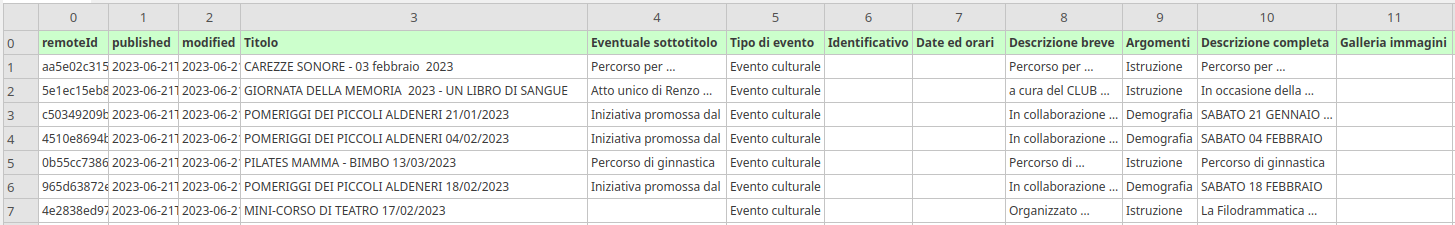
\includegraphics[width=1\linewidth]{knowdive-files/raw_dataset.png}
    \caption{Raw dataset format}
    \label{fig:raw_data}
\end{figure}

\noindent Then, during the cleaning process, we resolved inconsistencies by removing duplicate entries and correcting formatting issues. Specifically, we eliminated numerous irrelevant attributes from the raw data, such as \textit{"published"} and \textit{"modified"}, as they were not essential for our project objectives. Additionally, we extracted useful information (such as dates, times, and locations) from the \textit{"descrizione completa"} field, where this data was often embedded. As shown in Figure \ref{fig:cleaned_data}, this meticulous cleaning process allowed us to reduce noise and significantly improve the overall quality and relevance of the dataset.
\begin{figure}[H]
    \centering
    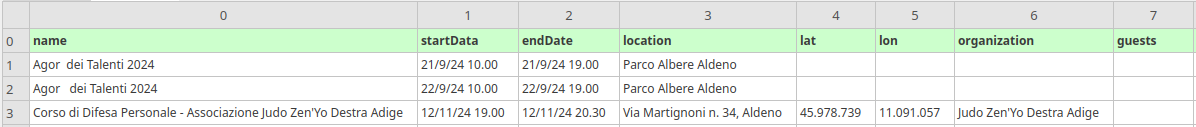
\includegraphics[width=1\linewidth]{knowdive-files/cleaned_dataset.png}
    \caption{Dataset after cleaning process}
    \label{fig:cleaned_data}
\end{figure}

\noindent Finally, we standardized the dataset to ensure consistency and compatibility with our project requirements. This involved restructuring key fields such as event names, dates, and locations to adhere to a uniform format. For instance, we standardized date entries to the format "YYYY-MM-DD HH:MM:SS" and ensured that all textual information was consistent in structure and style. 
\vspace{0.4cm}

\noindent Additionally, we conducted a "dataset integration" phase, where we linked related datasets to create meaningful connections. For example, we connected the Guest CSV with the Event CSV by associating the \textit{id} of each guest with the corresponding event instance. This step allowed us to establish relationships between datasets, enriching the overall data structure and improving its utility for our knowledge graph. As shown in Figure \ref{fig:standardized_data}, the event \textit{"ALESSANDRO COLOMBO: TAGLIATO PER VIVERE"} has the guest number \textit{8} which corresponds to \textit{"Alessandro Colombo"} in the Guest CSV in Figure \ref{fig:guest_csv} .

\begin{figure}[H]
    \centering
    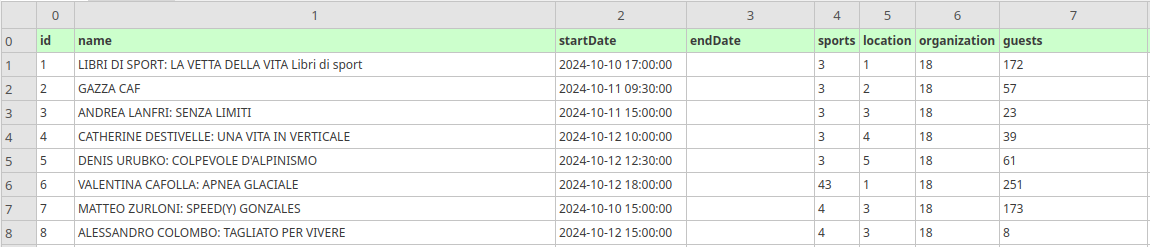
\includegraphics[width=1\linewidth]{knowdive-files/standardized_dataset.png}
    \caption{Dataset after standardization process}
    \label{fig:standardized_data}
\end{figure}
\begin{figure}
    \centering
    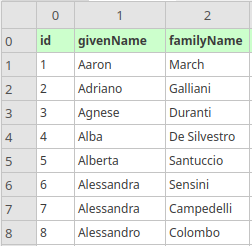
\includegraphics[width=0.23\linewidth]{knowdive-files/guest_dataset.png}
    \caption{Guest CSV}
    \label{fig:guest_csv}
\end{figure}

%-------------------------------------------------------------------------------------
\mycomment{
    In this section the second main input for the project is described, namely the data source list (if available). The resources (language, schema and data values) available as input for projects, has to be properly described. More in details for each resource has to be reported:
    \begin{itemize}
        \item The name, and the description of the information the resource is carrying.
        \item Type of resource. If it is a language, schema or data value dataset.
        \item The source from which such resource can be collected.
        \item If the resources is diversity-aware (thus already produced by iTelos) or needs to be improved in terms of diversity (i.e., data coming from low quality sources). 
    \end{itemize}
    
    Moreover, this section aims at reporting the execution of the activities involved in the Information Gathering iTelos phase.\\
    
    \noindent Information Gathering sub activities:
    \begin{itemize}
            \item Sources identification
            \item Datasets collection
            \item Datasets cleaning
            \item Datasets standardization
    \end{itemize}
    
    
    \noindent The report of the work done during the first phase of the methodology, has to includes also the description of the different choices made, with their strong and weak points. In other words the report should provide to the reader, a clear description of the reasoning conducted by all the different team members.
}
\section{Language Definition}
\noindent In the Language Definition phase, the focus is on adapting the language, i.e. word and concepts, required to accurately represent the information and relationships within our Knowledge Graph (KG). This phase builds upon the outputs of previous phases, such as the Purpose Formalization Sheet, Entity-Relationship (ER) Model, and the resource set. It aims to create a purpose-specific language that connects the project's goals with the data's conceptual representation.
\vspace{0.4cm}

\noindent The objective is to ensure that the concepts used are aligned with the project’s goals and effectively represent the data’s entity types (ETypes), attributes, and relationships. This is achieved by leveraging existing ontologies and vocabularies to identify standardized definitions. A cascade approach is applied in this process: first, each concept is checked for its presence in the \href{https://ukc.datascientia.eu/concept}{\textbf{Universal Knowledge Core (UKC)}}. If the concept is not found in the UKC or does not align with the project’s requirements, alternative sources such as \href{https://schema.org}{\textbf{schema.org}} and \href{https://wiki.openstreetmap.org/wiki/Map_features}{\textbf{OpenStreetMap wiki}} are consulted. If the concept remains undefined, a new ConceptID is created, following a structured format such as \texttt{KGE24-SportFacilities\&SportEvents-8XXX}. In this phase, it is important to note that it was not possible to create fully automated scripts to extract these language definitions. This is because each word had to be carefully reviewed from both a grammatical and semantic perspective to ensure it aligns with the project's characteristics. For example, if we take the entity "\textit{Guest}", the UKC provides us with the same word but with a meaning that differs from the one given in this project. Alternatively, when looking at "\textit{celebrity}" in UKC, the meaning partially reflects that of "\textit{Guest}" (in the project's context), but the word itself does not align. This is also a particular case, as it is not possible to find a perfect semantic and grammatical match in any resource. The definition of "\textit{Guest}" is a custom language definition uniquely created for this project.
\vspace{0.4cm}

\noindent To establish a structured and coherent language definition, we organize the information into three distinct tables:
\begin{itemize}
    \item Table \ref{tab:table1}: Dedicated to Entity Types (ETypes).
    \item Table \ref{tab:table2}: Focused on relationships.
    \item Table \ref{tab:table3}: Covering attributes.
\end{itemize}

\noindent In conclusion, by the end of this phase, all entities, relationships, and attributes in the KG will adhere to the newly formalized vocabulary. This guarantees consistency and clarity in how information is represented.

\vspace{-7pt}
\begin{table}[H]
    \centering
    \renewcommand{\arraystretch}{1.5} % Adjust row height for better vertical centering
    \begin{tabularx}{\textwidth}{|M{3cm}|M{3cm}|X|}
        \hline
        \textbf{ConceptID} & \textbf{Word-en} & \textbf{Gloss-en} \\ \hline
        UKC-2593 & sport & An active diversion requiring physical exertion and competition.\\ \hline
        UKC-17619 & facility & A building or place that provides a particular service or is used for a particular industry.\\ \hline
        UKC-56 & event & Something that happens at a given place and time.\\ \hline
        UKC-43416 & organization & The persons (or committees or departments etc.) who make up a body for the purpose of administering something.\\ \hline
        UKC-695 & location & The persons (or committees or departments etc.) who make up a body for the purpose of administering something.\\ \hline
        UKC-53492 & user & A person who makes use of a thing; someone who uses or employs something.\\ \hline
        KGE24-SportFacilities\linebreak\&SportEvents-8001 & Guest & Represents a guest or participant involved in a sports event.\\ \hline
        KGE24-SportFacilities\linebreak\&SportEvents-8002 & PadelCourt & A court dedicated to padel, a racquet sport.\\ \hline
        KGE24-SportFacilities\linebreak\&SportEvents-8003 & TennisCourt & A court dedicated to tennis.\\ \hline
        KGE24-SportFacilities\linebreak\&SportEvents-8004 & VolleyballField & A field dedicated to volleyball.\\ \hline
    \end{tabularx}
    \caption{EType concept labels and descriptions.}
    \label{tab:table1}
\end{table}

\begin{table}[H]
    \centering
    \renewcommand{\arraystretch}{1.5} % Adjust row height for better vertical centering
    \begin{tabularx}{\textwidth}{|M{3cm}|M{3cm}|X|}
        \hline
        \textbf{ConceptID} & \textbf{Word-en} & \textbf{Gloss-en}.\\ \hline
        UKC-85982 & placed & Situated in a particular spot or position.\\ \hline
        UKC-104711  & organise & Create (as an entity).\\ \hline
        UKC-101132 & appear  & Character on stage or appear in a play, etc.\\ \hline
        UKC-97761  & play & Participate in games or sport.\\ \hline
        UKC-105477 & attend & Be present at (meetings, church services, university), etc.\\ \hline
        UKC-92536  & basedOn & Being derived from (often followed by 'on' or 'upon').\\ \hline
        UKC-103527  & have & Have or possess, either in a concrete or an abstract sense.\\ \hline
    \end{tabularx}
    \caption{Relationships concept labels and descriptions.}
    \label{tab:table2}
\end{table}

\begin{table}[H]
    \centering
    \renewcommand{\arraystretch}{1.5} % Adjust row height for better vertical centering
    \begin{tabularx}{\textwidth}{|M{3cm}|M{3cm}|X|}
        \hline
        \textbf{ConceptID} & \textbf{Word-en} & \textbf{Gloss-en}.\\ \hline
        UKC-36247 & identification & Evidence of identity; something that identifies a person or thing (full form of "\textit{id}").\\ \hline
        UKC-33531 & given\_name & The name that precedes the surname.\\ \hline
        UKC-33528 & family\_name & The name used to identify the members of a family (as distinguished from each member's given name).\\ \hline
        schema.org-birthDate & birthDate & Date of birth.\\ \hline
        schema.org-hasOccupation & hasOccupation & The person's occupation.\\ \hline
        UKC-2 & name & A language unit by which a person or thing is known.\\ \hline
        schema.org-startDate & startDate & The start date and time of the item.\\ \hline
        schema.org-endDate & endDate & The end date and time of the item.\\ \hline
        UKC-45004 & address & The place where a person or organization can be found or communicated with.\\ \hline
        UKC-45537 & municipality & An urban district having corporate status and powers of self-government.\\ \hline
        OSM-surface & surface & Describes the surface of a feature.\\ \hline
        UKC-75466 & lit & Provided with artificial light.\\ \hline
        UKC-83504 & covered & Overlaid or spread or topped with or enclosed within something; sometimes used as a combining form.\\ \hline
    \end{tabularx}
    \caption{Data properties concept labels and descriptions.}
    \label{tab:table3}
\end{table}


%-------------------------------------------------------------------------------------
\mycomment{    
    This section is dedicated to the description of the Language Definition phase. Like in the previous section, it aims to describe the different sub activities performed by all the team members, as well as the phase outcomes produced.\\
    
    
    \noindent Language Definition sub activities:
    \begin{itemize}
        \item Concept identification
        \item Dataset filtering
    \end{itemize}
    
    
    \noindent The report of the work done during this phase of the methodology, has to includes also the description of the  different choices made, with their strong and weak points. In other words the report should provide to the reader, a clear description of the reasoning conducted by all the different team members.
}
\section{Knowledge Definition}

% -----------------------------------------------------------------------------------------------------
\mycomment{
    This section is dedicated to the description of the Knowledge Definition phase. Like in the previous section, it aims to describe the different sub activities performed by all the team members, as well as the phase outcomes produced.\\
    
    
    
    \noindent Knowledge Definition sub activities:    
        \begin{itemize}
            \item KTelos
            \begin{itemize}
                \item Teleology definition
                \item Teleontology definition
            \end{itemize}
            \item Dataset cleaning and formatting
        \end{itemize}
    
    
    \noindent The report of the work done during this phase of the methodology, has to includes also the description of the  different choices made, with their strong and weak points. In other words the report should provide to the reader, a clear description of the reasoning conducted by all the different team members.
}
%\section{Entity Definition}

This section is dedicated to the description of the Entity Definition phase. Like in the previous section, it aims to describe the different sub activities performed by all the team members, as well as the phase outcomes produced. 


\noindent Entity Definition sub activities:
\begin{itemize}
        \item Entity matching
        \item Entity identification 
        \item Data mapping
\end{itemize}

\noindent The report of the work done during this phase of the methodology, has to includes also the description of the  different choices made, with their strong and weak points. In other words the report should provide to the reader, a clear description of the reasoning conducted by all the different team members.


%\section{Evaluation}

This section aims at describing the evaluation performed at the end of the whole process over the final outcome of the iTelos methodology. More in details, this section as to report:

\begin{itemize}
    \item the final Knowledge Graph information statistics (like, number of etypes and properties, number of entities for each etype, and so on).
    \item Knowledge layer evaluation: the results of the application of the evaluation metrics applied over the knowledge layer of the final KG.
    \item Data layer evaluation: the results of the application of the evaluation metrics applied over the data layer of the final KG.
    \item Query execution: the description of the competency queries executed over the final KG in order to test the suitability of the KG to satisfy the project purpose. 
\end{itemize}


%\section{Metadata Definition}

In this section the report collects the definitions of all the metadata defined for the different resources produced along the whole process. The metadata defined in this phase describes both the final outcome of the project, and the intermediate outcome of each phase (language, schema, and data source standardised values).\\

\noindent The definition of the metadata, is crucial to enable the distribution (sharing) of the resource produced, through the data catalogs. For this reason it is important to describe also where such metadata will be published to distribute the resources it describes (for example the DataScientia catalogs). \\

\noindent In particular the structure of this section is organized as follows, with the objective to describe the metadata relative to all the type of resources produced by the project.\\
\begin{itemize}
    \item Project metadata description
    \item Language resources metadata description
    \item Knowledge resources metadata description
    \item Data resources metadata description
\end{itemize}



%\section{Open Issues}

This section concludes the current document with final conclusions regarding the quality of the process and final outcome, and the description of the issues that (for lack of time or any other cause) remained open.\\

\begin{itemize}
    \item Did the project respect the scheduling expected in the beginning ?
    \item Are the final results able to satisfy the initial Purpose ?
        \begin{itemize}
            \item If no, or not entirely, why ? which parts of the Purpose have not been covered ?
        \end{itemize}
\end{itemize}


\noindent Moreover, this section aims to summarize the most relevant issues/problems remained open along the iTelos process. The description of open issues has to provide a clear explanation about the problems, the approaches adopted while trying to solve them and, eventually, any proposed solution that has not been applied.\\

\begin{itemize}
    \item which are the issues remained open at the end of the project ?
\end{itemize}

\end{spacing}
\end{sloppypar}
\end{document} 